\chapter{Introdução}

%Seções sugeridas:

%\section{Objetivos}

%\section{Descrição de composição e funcionamento do CPA/CPE}

%\subsection{Estrutura de Gestão}

%\subsection{Parcerias}

%\subsubsection{Órgãos Públicos}

%\subsubsection{Empresas}
\section{Enunciando do problema}
Empresas que produzem cerveja em pequena escala, conhecidas como microcervejarias ou cervejarias artesanais, diferenciam-se das grandes corporações multinacionais que operam com produção em larga escala. As microcervejarias se destacam por fabricar uma ampla variedade de estilos e sabores complexos, geralmente em lotes reduzidos \cite{garavaglia2018craft, elzinga2015craft}. Considerando que essas empresas geralmente dispõem de recursos limitados para investimentos em pesquisa e desenvolvimento, tecnologias como inteligência artificial e internet das coisas podem oferecer vantagens competitivas, especialmente por suas características de baixo custo \cite{dias2021cloud}. Pequenas e médias empresas devem, portanto, avaliar a adoção dessas novas tecnologias e acompanhar a tendência de transformação digital em seus processos \cite{teng2022sme}.

Dias et al.~\cite{dias2023microbrewery} destacam que o grau de automação nas microcervejarias ainda é reduzido, sendo necessárias melhorias para aumentar a transparência do processo produtivo. Além disso, diversos indicadores cruciais de desempenho não são monitorados ou o são de forma manual, o que pode resultar em imprecisões nos dados do processo.

Nesse cenário, este projeto de pesquisa tem como objetivo identificar o perfil e as necessidades das microcervejarias. A partir desse diagnóstico, pretende-se investigar e desenvolver arquiteturas de transformação digital aplicáveis ao processo produtivo, priorizando soluções de custo-efetivo.

Outra contribuição do projeto está na análise dos dados gerados, com o intuito de aproveitá-los de forma mais ampla, não apenas para monitoramento e controle de variáveis específicas, mas também para estimar outras variáveis e indicadores-chave de desempenho (KPIs), avaliar a saúde operacional do processo produtivo e promover sua otimização.

De forma geral, o projeto busca analisar o potencial dos sistemas de transformação digital para contribuir com a sustentabilidade dos processos produtivos em microcervejarias. Espera-se que tais sistemas promovam a otimização dos processos, reduzindo o tempo de cada etapa, o consumo de energia e os custos com manutenção, além de evitar perdas de produção e retrabalhos. Também se espera que contribuam para a melhoria da qualidade do produto final, um dos principais desafios enfrentados por esse tipo de empresa.

\section{Fundamentação teórica}
Nesta seção é apresentada a fundamentação teórica que sustenta o desenvolvimento do presente trabalho. São discutidos os principais conceitos relacionados à transformação digital e à Indústria~4.0, bem como as arquiteturas e tecnologias computacionais que viabilizam esses processos, com destaque para a computação em nuvem, a computação em névoa e a computação de borda. %O objetivo desta seção é fornecer o embasamento conceitual necessário para a compreensão das escolhas metodológicas e da abordagem adotada ao longo do projeto.

\subsection{Transformação digital, Indústria 4.0 e arquiteturas digitais}

A transformação digital tem se consolidado como um dos principais paradigmas contemporâneos de mudança organizacional e industrial, sendo compreendida como um processo que vai além da simples adoção de tecnologias digitais. De acordo com Vial \cite{vial2021understanding}, a transformação digital envolve mudanças profundas nas estruturas organizacionais, nos processos operacionais e nos modelos de negócio, nas quais tecnologias digitais atuam como elementos catalisadores de novas formas de criação, entrega e captura de valor. Nesse sentido, a digitalização não constitui um fim em si mesma, mas um meio para reconfigurar estratégias organizacionais e ampliar a capacidade adaptativa das empresas em ambientes competitivos e dinâmicos.

No contexto industrial, a transformação digital encontra sua expressão mais abrangente no paradigma da Indústria~4.0, frequentemente associada à chamada quarta revolução industrial. Ghobakhloo \cite{ghobakhloo2020industry} descreve a Indústria~4.0 como um processo de digitalização sistêmica da manufatura e das cadeias de valor, caracterizado pela integração entre sistemas físicos, digitais e humanos. Diferentemente das revoluções industriais anteriores, a Indústria~4.0 fundamenta-se na conectividade contínua, na interoperabilidade entre sistemas e na capacidade de tomada de decisão orientada por dados, viabilizando ambientes produtivos inteligentes e descentralizados.

Sob essa perspectiva, a Indústria~4.0 não deve ser interpretada apenas como um conjunto de tecnologias emergentes, mas como um sistema estruturado em princípios fundamentais, tais como interoperabilidade, integração horizontal e vertical, virtualização, descentralização e capacidade de operação em tempo real \cite{ghobakhloo2020industry}. Esses princípios sustentam a transformação digital industrial ao permitir que dados provenientes de diferentes etapas do processo produtivo sejam coletados, integrados e analisados de forma contínua, possibilitando maior eficiência operacional, flexibilidade produtiva e suporte avançado à tomada de decisão.

% Está um pouco repetitivo o que é dito nesse parágrafo e nos próximos três, ficar falando a mesma coisa sempre não agrega
Embora grande parte da literatura inicial sobre Indústria~4.0 tenha se concentrado em grandes corporações industriais, espera-se que a transformação digital também represente uma abordagem relevante para pequenas e médias empresas. Schallmo et al.~\cite{schallmo2017digital} argumentam que a transformação digital deve ser compreendida como um processo incremental e estratégico, no qual organizações de menor porte podem explorar tecnologias digitais de maneira progressiva, alinhando inovação tecnológica e viabilidade econômica. Nesse contexto, a transformação digital reduz barreiras historicamente associadas ao acesso a tecnologias avançadas, permitindo que empresas de menor escala adotem soluções que permitam resultados anteriormente restritas a grandes players industriais.

Esse aspecto é particularmente relevante no caso de microcervejarias e cervejarias artesanais, que operam em ambientes caracterizados por alta variabilidade de produtos, processos produtivos flexíveis e forte ênfase em qualidade e diferenciação. Apesar dessas características, tais empresas geralmente dispõem de recursos limitados para investimentos em automação pesada e infraestrutura tecnológica proprietária. A transformação digital, ao introduzir tecnologias mais acessíveis, modulares e baseadas em software, cria oportunidades para ganhos significativos em eficiência produtiva, controle de processos, rastreabilidade e suporte à tomada de decisão, sem a necessidade de investimentos incompatíveis com a realidade dessas organizações \cite{vial2021understanding,sestino2020internet}. % talvez citar algo mais específico

Sestino et al.~\cite{sestino2020internet} ressaltam que tecnologias digitais associadas à transformação digital, como plataformas computacionais, sistemas de coleta e análise de dados e soluções conectadas, possibilitam não apenas a digitalização de processos existentes, mas também a inovação em modelos de negócio. Assim, a transformação digital em pequenas e médias empresas pode ser entendida como um mecanismo de democratização tecnológica, 
ampliando o acesso a capacidades analíticas e operacionais que anteriormente demandavam infraestruturas complexas e de alto custo.

A materialização da transformação digital e dos princípios da Indústria~4.0 depende, contudo, da adoção de arquiteturas computacionais adequadas para coleta, processamento, armazenamento e análise de dados. Nesse contexto, arquiteturas digitais baseadas em computação em nuvem, computação em névoa (\textit{fog computing}) e computação de borda (\textit{edge computing}) têm assumido papel central como infraestruturas habilitadoras da digitalização industrial. A computação em nuvem destaca-se por oferecer recursos computacionais escaláveis, acessíveis sob demanda e com modelos de custo flexíveis, viabilizando a centralização de dados, a integração de sistemas e o desenvolvimento de serviços digitais \cite{armbrust2010view,cloud2011nist}.

Entretanto, conforme apontado por Ghobakhloo \cite{ghobakhloo2020industry}, a transformação digital industrial impõe requisitos específicos relacionados à latência, confiabilidade e operação em tempo real, que nem sempre são plenamente atendidos por arquiteturas exclusivamente centralizadas. Esses requisitos tornam-se particularmente relevantes em ambientes produtivos, nos quais decisões operacionais precisam ser tomadas de forma rápida e robusta, mesmo diante de limitações de conectividade ou falhas de comunicação. Nesse cenário, abordagens baseadas em computação de borda e computação em névoa emergem como complementares à computação em nuvem, ao possibilitar o processamento descentralizado de dados próximo à fonte de geração da informação.

Assim, arquiteturas híbridas que combinam computação em nuvem, fog e edge computing têm sido amplamente discutidas na literatura como soluções capazes de equilibrar centralização e descentralização, escalabilidade e responsividade, bem como integração global e autonomia local. Essas arquiteturas alinham-se diretamente aos princípios da Indústria~4.0, em especial à descentralização e à capacidade de operação em tempo real, constituindo a base tecnológica sobre a qual processos de transformação digital podem ser implementados de forma eficaz e sustentável, inclusive em sistemas produtivos de pequena escala.



\subsection{Computação em nuvem (Cloud Computing)}
% =========================================================
% Cloud Computing
% Referências principais:
% - Armbrust et al. (2010): visão fundacional e trade-offs
% - Mell & Grance (2011): definição formal (NIST) e modelos
% - Marston et al. (2011): implicações de negócio e adoção
% - Ghobakhloo (2020): cloud como habilitador de Indústria 4.0
% =========================================================

% !!!!!!!!!!!!!!!!!!!!!!!!!!!!!!!!!!!!!!!!!!!!!!!!!!!!!!!!!
% TODOs:
% - Colocar palavras em inglês em itálico
% - Revisar o tamanho do texto
% !!!!!!!!!!!!!!!!!!!!!!!!!!!!!!!!!!!!!!!!!!!!!!!!!!!!!!!!!

A computação em nuvem (\textit{cloud computing}) consolidou-se como um dos pilares tecnológicos da transformação digital ao viabilizar o acesso ubíquo a recursos computacionais sob demanda, com elasticidade e modelos de cobrança baseados em uso. Uma definição amplamente adotada é a proposta pelo NIST, que descreve a computação em nuvem como um modelo que permite acesso conveniente e onipresente, via rede, a um conjunto compartilhado de recursos configuráveis (por exemplo, redes, servidores, armazenamento, aplicações e serviços), que podem ser rapidamente provisionados e liberados com mínimo esforço de gerenciamento ou interação com o provedor \cite{cloud2011nist}. Em termos práticos, esse paradigma desloca a aquisição tradicional de infraestrutura (CAPEX) para um modelo predominantemente operacional (OPEX), acelerando a experimentação e a escalabilidade de sistemas digitais \cite{armbrust2010view}.

\subsubsection{Características essenciais e modelos de serviço}
A caracterização do NIST explicita propriedades que diferenciam a nuvem de abordagens anteriores de terceirização de TI: (i) autosserviço sob demanda; (ii) amplo acesso via rede; (iii) compartilhamento de recursos (multitenancy); (iv) elasticidade rápida; e (v) serviço mensurado \cite{cloud2011nist}. Essas propriedades estão diretamente relacionados com as vantagens do uso da computação a nuvem, que serão discutidas adiante, além disso sustentam três modelos de serviço, frequentemente utilizados para organizar a discussão arquitetural e de governança:
\begin{itemize}
    \item \textbf{IaaS} (\textit{Infrastructure as a Service}): fornece infraestrutura virtualizada (máquinas, redes, armazenamento), permitindo ao usuário gerenciar sistemas operacionais e aplicações.
    \item \textbf{PaaS} (\textit{Platform as a Service}): oferece uma plataforma gerenciada (runtime, middleware, banco de dados), reduzindo o esforço operacional do usuário.
    \item \textbf{SaaS} (\textit{Software as a Service}): disponibiliza aplicações completas como serviço, com mínima gestão por parte do usuário final.
\end{itemize}
Além disso, são comuns modelos de implantação \textbf{pública}, \textbf{privada}, \textbf{comunitária} e \textbf{híbrida} \cite{cloud2011nist}. Para aplicações industriais, arquiteturas híbridas são frequentemente motivadas por requisitos de conformidade, sensibilidade de dados e necessidades de integração com sistemas legados, ao mesmo tempo em que preservam a elasticidade e a escalabilidade da nuvem pública.

\subsubsection{Nuvem como habilitador da transformação digital e da Indústria 4.0}
No contexto da Indústria~4.0, a nuvem atua como infraestrutura integradora para agregação e processamento de dados provenientes de sensores, máquinas, sistemas de execução da manufatura (MES), sistemas de gestão (ERP) e demais componentes da cadeia de valor. Em revisões sobre Indústria~4.0, a computação em nuvem aparece como uma tecnologia habilitadora recorrente, associada à integração vertical e horizontal, à interoperabilidade e ao suporte a análises avançadas (por exemplo, \textit{big data analytics} e inteligência artificial) \cite{ghobakhloo2020industry}. Em particular, a capacidade de concentrar dados de múltiplas fontes, padronizar interfaces e escalar recursos computacionais sob demanda viabiliza o desenvolvimento de serviços digitais, monitoração remota, rastreabilidade e suporte decisório orientado a dados em tempo quase real, alinhando-se a princípios como capacidade em tempo real e integração ao longo da cadeia \cite{ghobakhloo2020industry}.

Do ponto de vista organizacional, a nuvem também favorece a adoção incremental de soluções digitais, pois reduz barreiras de entrada associadas à aquisição e manutenção de infraestrutura local. Esse aspecto é relevante para pequenas e médias empresas que buscam iniciar jornadas de transformação digital com investimentos graduais e maior flexibilidade para testar aplicações (por exemplo, \textit{dashboards}, análise de qualidade, gestão de manutenção e controle de processos), preservando a possibilidade de evolução futura \cite{armbrust2010view,marston2011cloud}.

\subsubsection{Vantagens: escalabilidade, agilidade e centralização de dados}
Entre as principais vantagens da computação em nuvem, destacam-se:
\begin{enumerate}
    \item \textbf{Elasticidade e escalabilidade}: capacidade de ajustar recursos rapidamente conforme variação de carga, reduzindo sub ou superdimensionamento \cite{armbrust2010view}.
    \item \textbf{Agilidade e \textit{time-to-market}}: provisionamento rápido acelera prototipação e implantação de sistemas digitais \cite{armbrust2010view,marston2011cloud}.
    \item \textbf{Centralização e integração de dados}: consolidação de fontes heterogêneas facilita análises globais, auditorias e rastreabilidade \cite{cloud2011nist}.
    \item \textbf{Economias de escala}: provedores podem otimizar utilização e custos energéticos/operacionais, repassando parte do ganho ao usuário \cite{armbrust2010view}.
\end{enumerate}

\subsubsection{Limitações e trade-offs: latência, conectividade, segurança e lock-in}
Apesar de seus benefícios, a nuvem impõe limitações relevantes, especialmente em cenários industriais e ciberfísicos:
\begin{enumerate}
    \item \textbf{Latência e variabilidade de rede}: aplicações de controle e resposta rápida podem ser sensíveis a atrasos e jitter, o que limita o envio de todos os dados e decisões exclusivamente para a nuvem \cite{armbrust2010view}.
    \item \textbf{Dependência de conectividade}: interrupções de rede podem degradar serviços críticos se não houver mecanismos locais de contingência.
    \item \textbf{Segurança, privacidade e conformidade}: a centralização de dados e o multitenancy ampliam preocupações com confidencialidade, integridade e governança; tais aspectos influenciam decisões por nuvens privadas/híbridas \cite{cloud2011nist}.
    \item \textbf{\textit{Vendor lock-in}}: dependência de APIs proprietárias e serviços gerenciados pode aumentar custos de migração e reduzir flexibilidade futura, configurando um trade-off frequente na adoção de PaaS/SaaS \cite{armbrust2010view,marston2011cloud}.
\end{enumerate}
Esses trade-offs não anulam o valor da nuvem; ao contrário, motivam arquiteturas distribuídas e híbridas, nas quais parte do processamento ocorre próximo à fonte de dados (conceitos aprofundados nas subseções de \textit{fog} e \textit{edge computing}). Em ambientes de Indústria~4.0, essa discussão conecta-se diretamente ao princípio de descentralização e à necessidade de decisões operacionais locais para manter desempenho e robustez, enquanto a nuvem permanece como camada de integração, histórico e análises globais \cite{ghobakhloo2020industry}.



\subsection{Computação em névoa (Fog Computing)}
% =========================================================
% Fog Computing (texto exaustivo para base de artigo)
% Referências principais sugeridas:
% - Bonomi et al. (2012): introdução do conceito de fog computing
% - Mouradian et al. (2018): survey abrangente sobre fog computing
% - Chiang & Zhang (2016): fog computing para IoT e aplicações tempo-críticas
% - Ghobakhloo (2020): requisitos de descentralização e tempo real na Indústria 4.0
% =========================================================

A computação em névoa (\textit{fog computing}) emerge como um paradigma arquitetural distribuído que estende capacidades de processamento, armazenamento e comunicação para camadas intermediárias entre a computação em nuvem e os dispositivos finais. O termo foi introduzido por Bonomi et al.~\cite{bonomi2012fog} com o objetivo de atender às limitações de latência, confiabilidade e consciência de contexto observadas em arquiteturas puramente centralizadas, especialmente em aplicações baseadas em Internet das Coisas (IoT) e sistemas ciberfísicos.

Enquanto a computação em nuvem concentra recursos computacionais em grandes centros de dados, a computação em névoa propõe uma hierarquia de nós distribuídos, denominados \textit{fog nodes}, que podem incluir gateways industriais, servidores locais, roteadores inteligentes e controladores industriais com capacidade computacional. Esses nós são posicionados logicamente próximos às fontes de dados e atuam como intermediários inteligentes, realizando tarefas de pré-processamento, agregação e análise inicial antes do encaminhamento seletivo das informações para camadas superiores \cite{bonomi2012fog,mouradian2017comprehensive}.

Do ponto de vista arquitetural, a computação em névoa não substitui a computação em nuvem, mas a complementa. A nuvem permanece responsável por tarefas de maior complexidade computacional, armazenamento histórico, aprendizado de máquina em larga escala e análises globais, enquanto a névoa atende aplicações sensíveis a tempo, que demandam respostas rápidas e processamento contextualizado. Essa separação funcional permite equilibrar escalabilidade e desempenho, especialmente em sistemas distribuídos e heterogêneos \cite{mouradian2017comprehensive,chiang2016fog}.

No contexto da transformação digital industrial e da Indústria~4.0, a computação em névoa apresenta forte alinhamento com princípios como descentralização, integração vertical e capacidade de operação em tempo real. Ghobakhloo \cite{ghobakhloo2020industry} destaca que ambientes industriais digitalizados requerem arquiteturas capazes de suportar decisões locais e autônomas, reduzindo a dependência de infraestruturas centralizadas e aumentando a resiliência operacional. A computação em névoa atende a esses requisitos ao permitir que eventos críticos sejam tratados localmente, preservando desempenho mesmo diante de instabilidades de rede ou restrições de conectividade.

Entre as principais vantagens associadas à computação em névoa, destacam-se:
\begin{enumerate}
    \item \textbf{Redução de latência}: o posicionamento intermediário dos recursos computacionais permite tempos de resposta significativamente menores em comparação com arquiteturas baseadas exclusivamente em nuvem \cite{bonomi2012fog,chiang2016fog}.
    \item \textbf{Eficiência no uso de banda}: a filtragem e agregação de dados na camada de névoa reduzem o volume de informações transmitidas para a nuvem, mitigando gargalos de comunicação \cite{mouradian2017comprehensive}.
    \item \textbf{Consciência de contexto}: a proximidade com o ambiente físico permite que decisões sejam tomadas com base em informações locais, como estado de máquinas, condições operacionais e eventos instantâneos.
    \item \textbf{Maior robustez operacional}: a capacidade de processamento local contribui para a continuidade de operação mesmo em cenários de falhas ou degradação da conectividade com a nuvem.
\end{enumerate}


\subsection{Computação de borda (Edge Computing)}
% =========================================================
% Edge Computing (texto exaustivo para base de artigo)
% Referências principais sugeridas:
% - Shi et al. (2016): visão fundacional e desafios do edge computing
% - Satyanarayanan et al. (2017): edge analytics e proximidade com a fonte
% - Mouradian et al. (2018): distinção conceitual entre cloud, fog e edge
% - Ghobakhloo (2020): requisitos industriais de tempo real e descentralização
% =========================================================

A computação de borda (\textit{edge computing}) representa um paradigma arquitetural que desloca capacidades de processamento, armazenamento e tomada de decisão para o ponto mais próximo possível da fonte de geração dos dados, isto é, para os próprios dispositivos finais ou para nós imediatamente adjacentes a eles. Diferentemente da computação em nuvem, que se baseia na centralização de recursos computacionais, e da computação em névoa, que introduz camadas intermediárias distribuídas, a computação de borda enfatiza o processamento \emph{no extremo da rede}, onde dados são produzidos e ações são executadas \cite{shi2016edge}.

Shi et al.~\cite{shi2016edge} definem edge computing como uma abordagem que visa reduzir latência, consumo de banda e dependência de conectividade por meio do processamento local ou quase local dos dados. Nesse paradigma, dispositivos como sensores inteligentes, controladores industriais, sistemas embarcados e computadores industriais desempenham papel ativo não apenas na coleta, mas também na análise e na resposta aos eventos observados. Essa proximidade física e lógica com o processo produtivo confere à computação de borda características singulares em termos de responsividade e determinismo temporal.

Do ponto de vista conceitual, é fundamental distinguir o escopo da computação de borda daquele atribuído à computação em névoa. Embora ambos os paradigmas compartilhem o objetivo de reduzir dependência de infraestruturas centralizadas, a computação em névoa posiciona recursos computacionais em \emph{camadas intermediárias}, como gateways e servidores locais, enquanto a computação de borda desloca o processamento diretamente para os dispositivos finais ou seus controladores imediatos \cite{mouradian2017comprehensive}. Assim, enquanto a névoa atua como um elo intermediário entre borda e nuvem, a borda representa o limite extremo da descentralização computacional.

Essa distinção explica a sobreposição conceitual frequentemente observada na literatura e na prática industrial. Em muitos sistemas, funcionalidades atribuídas informalmente à computação de borda são, na realidade, implementadas em camadas de névoa. A diferenciação adequada entre esses paradigmas permite maior clareza arquitetural e evita ambiguidades na definição de responsabilidades entre dispositivos, gateways e plataformas em nuvem \cite{mouradian2017comprehensive}.

No contexto da transformação digital industrial e da Indústria~4.0, a computação de borda apresenta forte alinhamento com requisitos de tempo real, confiabilidade e autonomia operacional. Ghobakhloo \cite{ghobakhloo2020industry} destaca que ambientes industriais digitalizados demandam decisões rápidas e locais, muitas vezes incompatíveis com atrasos introduzidos por arquiteturas centralizadas. A computação de borda atende a esses requisitos ao permitir que eventos críticos sejam processados e respondidos localmente, minimizando latência e garantindo continuidade operacional mesmo em cenários de conectividade limitada.

Entre as principais vantagens associadas à computação de borda, destacam-se:
\begin{enumerate}
    \item \textbf{Latência mínima}: o processamento ocorre no ponto de geração dos dados, permitindo respostas quase imediatas em aplicações críticas \cite{shi2016edge}.
    \item \textbf{Autonomia operacional}: sistemas de borda podem operar de forma independente da nuvem, aumentando robustez e resiliência.
    \item \textbf{Privacidade e segurança}: dados sensíveis podem ser processados localmente, reduzindo a necessidade de transmissão para camadas superiores \cite{satyanarayanan2015edge}.
    \item \textbf{Eficiência energética e de comunicação}: a redução no volume de dados transmitidos contribui para menor consumo de banda e energia.
\end{enumerate}

\subsection{Arquiteturas híbridas cloud--fog--edge como habilitadoras da transformação digital}

A adoção isolada de computação em nuvem, computação em névoa ou computação de borda raramente atende, de forma plena, aos requisitos impostos por processos de transformação digital em ambientes produtivos reais. Em especial no contexto industrial, a literatura tem convergido para o entendimento de que arquiteturas híbridas, que integram de forma coordenada essas três camadas computacionais, oferecem uma solução mais robusta, escalável e alinhada aos princípios da Indústria~4.0 \cite{armbrust2010view,bonomi2012fog,shi2016edge,ghobakhloo2020industry}. A Figura~\ref{fig:cloud_fog_edge} ilustra essa organização hierárquica, destacando o papel complementar desempenhado por cada camada.

\begin{figure}[h]
    \centering
    \caption{Arquitetura hierárquica cloud--fog--edge, evidenciando a distribuição de recursos computacionais e a escala de dispositivos em cada camada.}
    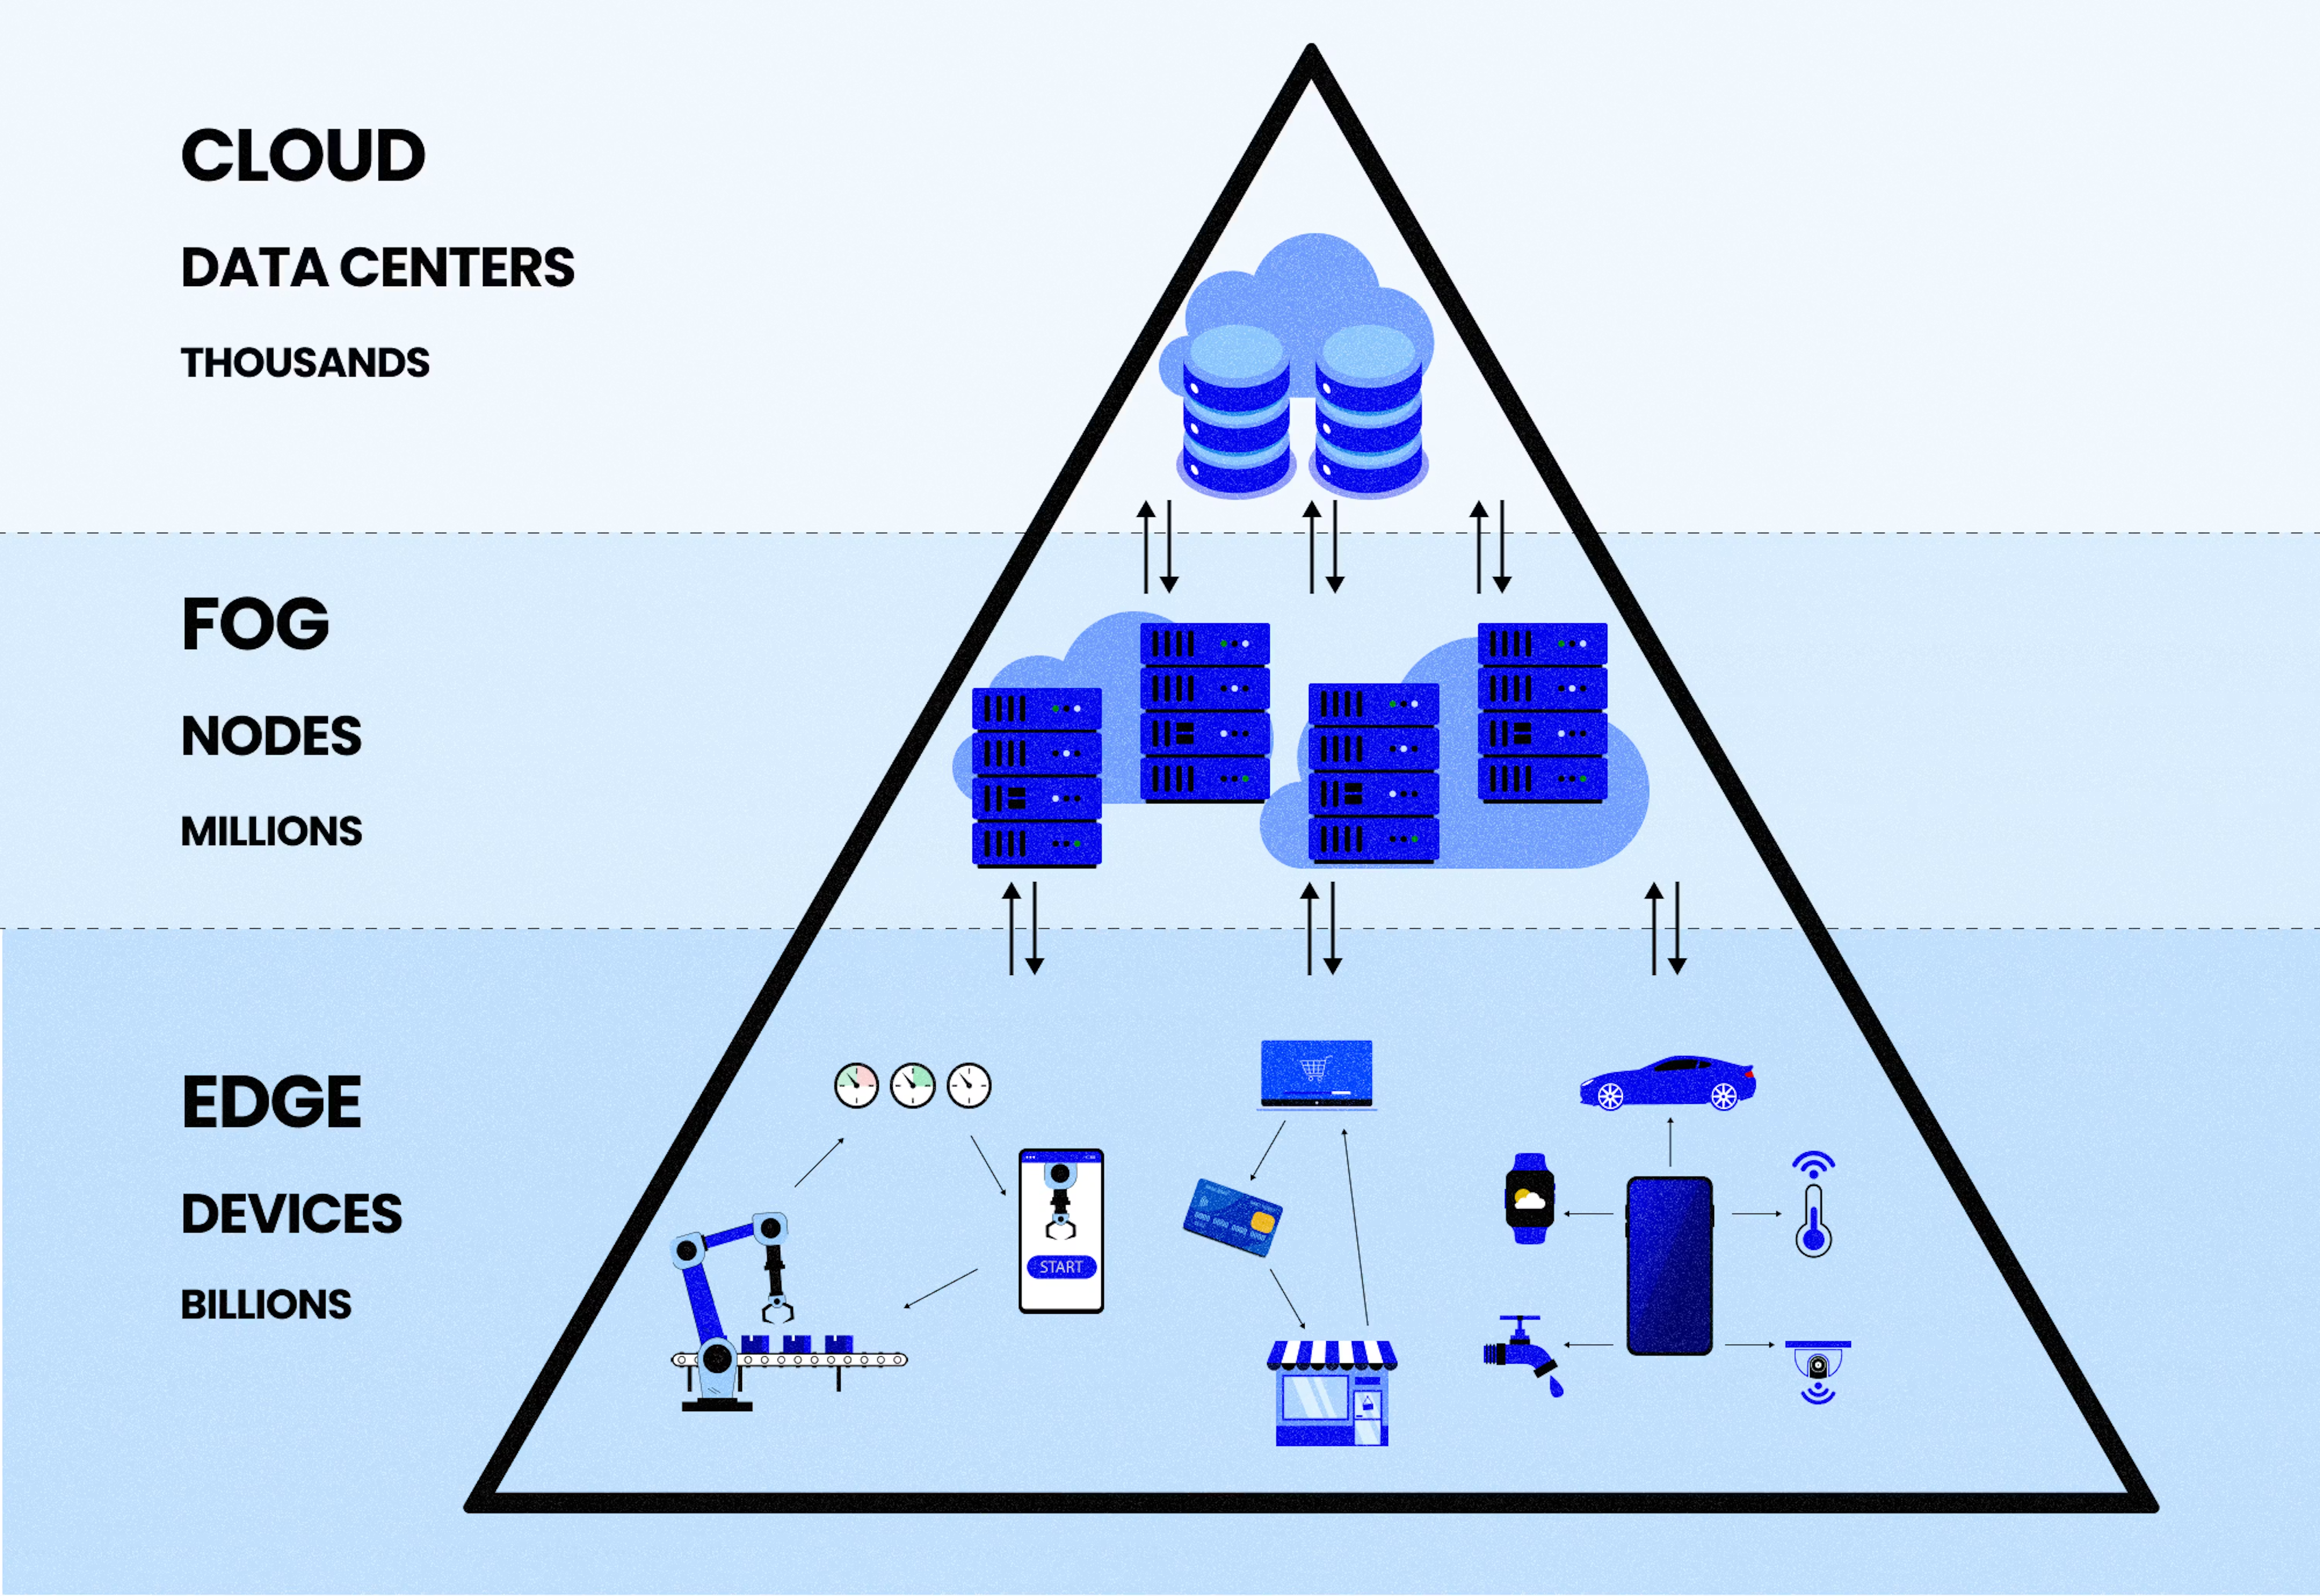
\includegraphics[width=0.7\textwidth]{./Figuras/cloud_edge_fog.png}
    \caption*{\small{Fonte: \url{https://maddevs.io/glossary/edge-computing/}}}
    \label{fig:cloud_fog_edge}
\end{figure}

Na camada superior, a computação em nuvem concentra grandes centros de dados responsáveis por armazenamento histórico, análises em larga escala, treinamento de modelos de aprendizado de máquina e integração global de informações. Essa camada oferece elevada capacidade computacional e elasticidade, sendo fundamental para consolidação de dados provenientes de múltiplas unidades produtivas, suporte à tomada de decisão e desenvolvimento de serviços digitais \cite{armbrust2010view,cloud2011nist}. Entretanto, sua dependência de conectividade e a latência associada à comunicação remota limitam sua aplicação direta em tarefas sensíveis a tempo.

A camada intermediária, associada à computação em névoa, atua como elo entre a nuvem e os dispositivos finais. Gateways industriais, servidores locais ou infraestruturas computacionais distribuídas realizam funções de agregação, filtragem, validação e análise inicial dos dados, reduzindo o volume de informações transmitidas para a nuvem e melhorando a responsividade do sistema \cite{bonomi2012fog,mouradian2017comprehensive}. Essa camada é particularmente relevante para coordenação de múltiplos dispositivos, integração de sistemas heterogêneos e manutenção da operação mesmo em cenários de conectividade intermitente.

Na base da arquitetura, a computação de borda posiciona capacidades computacionais diretamente nos dispositivos finais ou em seus controladores imediatos, permitindo monitoramento em tempo real, controle local e respostas quase instantâneas a eventos do processo físico \cite{shi2016edge,satyanarayanan2015edge}. Embora dispositivos de borda possuam recursos computacionais limitados, sua proximidade com o processo produtivo garante baixa latência, autonomia operacional e maior robustez frente a falhas de comunicação com camadas superiores.

Quando integradas de forma coerente, essas três camadas permitem distribuir responsabilidades computacionais de acordo com requisitos funcionais, temporais e organizacionais. Em pequenas e médias empresas, como microcervejarias, essa abordagem possibilita a implementação gradual da transformação digital, explorando tecnologias acessíveis e modulares. Dispositivos de borda podem ser utilizados para coleta de dados e controle local de processos; camadas de névoa podem realizar pré-processamento, monitoramento e integração de sistemas; enquanto a nuvem pode concentrar armazenamento histórico, visualização de indicadores, análises avançadas e suporte à tomada de decisão gerencial.

Essa arquitetura híbrida reduz barreiras tecnológicas historicamente associadas à digitalização industrial, permitindo que empresas de menor porte adotem práticas alinhadas à Indústria~4.0 sem a necessidade de infraestruturas complexas ou investimentos elevados. 
%Assim, a combinação coordenada de computação em nuvem, névoa e borda constitui um elemento central para viabilizar a transformação digital em contextos industriais distribuídos, flexíveis e orientados a dados, reforçando o caráter democrático e escalável desse paradigma tecnológico.

\section{Objetivos}
Considerando o baixo nível de digitalização observado em microcervejarias, bem como
a subutilização dos dados gerados nos processos industriais, especialmente em pequenas e
médias empresas, os objetivos deste projeto de pesquisa são:
\begin{itemize}
    \item verificar e analisar, junto às microcervejarias brasileiras e às indicadas pela VLB na Alemanha, a infraestrutura e os equipamentos atualmente disponíveis que sejam capazes de fornecer dados do processo produtivo;

    \item levantar as necessidades relacionadas às variáveis e aos indicadores-chave de desempenho (KPIs) mais relevantes para o monitoramento e controle do processo industrial;

    \item estimar os valores que as microcervejarias estão dispostas a investir em tecnologias digitais, em comparação com as soluções atualmente disponíveis no mercado.
\end{itemize}

Realizada essas etapas, o projeto visa investigar arquiteturas de transformação digital aplicáveis ao processo industrial dessas empresas, de forma a atender às suas necessidades específicas com soluções que sejam custo-efetivas.

\section{Descrição de composição e funcionamento do CPA/CPE}

O presente projeto de iniciação científica está sendo desenvolvido no campus Sertãozinho do Instituto Federal de Educação, Ciência e Tecnologia de São Paulo (IFSP), instituição pública de ensino, pesquisa e extensão com atuação voltada para formação técnica e científica. A localização do campus em Sertãozinho-SP confere uma posição vantajosa para o desenvolvimento de pesquisas aplicadas ao setor cervejeiro, uma vez que o município integra a região conhecida como Polo Cervejeiro de Ribeirão Preto, caracterizada pela concentração de microcervejarias, cervejarias artesanais e empresas associadas à cadeia produtiva da cerveja.

Essa proximidade geográfica com o setor produtivo cria condições favoráveis para a realização de estudos , análises comparativas e projetos de inovação tecnológica, permitindo a interação entre a academia e as empresas do setor. No contexto deste projeto, tal característica é particularmente relevante, pois possibilita a investigação de processos produtivos reais e a avaliação de estratégias de transformação digital em ambientes industriais de pequena e média escala.

O campus Sertãozinho do IFSP dispõe de infraestrutura laboratorial especializada voltada ao setor cervejeiro, destacando-se o Laboratório de Produção Cervejeira, o Laboratório de Microbiologia e o Centro Multidisciplinar de Tecnologia Cervejeira. Esses ambientes contam com equipamentos e recursos adequados para a produção de cervejas em escala laboratorial e experimental, bem como para a realização de análises físico-químicas e microbiológicas de cervejas e de suas matérias-primas.

\subsection{Estrutura de Gestão}

A condução do projeto ocorre de forma integrada à estrutura acadêmica e de pesquisa do campus Sertãozinho do IFSP. A equipe local é composta por dois professores pesquisadores, responsáveis pela orientação científica e pela supervisão das atividades desenvolvidas, além de dois estudantes de iniciação científica, que atuam na execução das etapas do projeto, incluindo levantamento de dados, análises comparativas e desenvolvimento das atividades propostas.

A estrutura de gestão conta com reuniões periódicas para acompanhamento das atividades, discussão dos resultados parciais e definição dos próximos passos, dinâmica que favorece a formação científica dos estudantes envolvidos e garante o alinhamento do projeto com os objetivos institucionais de pesquisa aplicada e inovação tecnológica do IFSP.

Adicionalmente, o projeto conta com o apoio de um pesquisador alemão, que atua como colaborador externo, contribuindo com sua experiência e auxiliando na troca de conhecimentos relacionados a práticas industriais, pesquisa aplicada e transformação digital no setor cervejeiro, além de realizar uma ponte para diferentes instituições alemãs.

\subsection{Parcerias}

O desenvolvimento do projeto é sustentado por parcerias que fortalecem sua relevância científica e tecnológica. Essas parcerias incluem tanto instituições de pesquisa internacionais quanto a interação potencial com empresas do setor cervejeiro local, criando um ambiente propício para a troca de conhecimentos e a validação das análises realizadas.

\subsubsection{Órgãos Públicos}

Como instituição pública federal, o IFSP desempenha papel importante no fomento à pesquisa, à inovação e à extensão tecnológica. A execução deste projeto está alinhada à missão institucional do IFSP de promover o desenvolvimento científico e tecnológico com impacto social e econômico, especialmente em regiões com vocação industrial específica, como o Polo Cervejeiro de Ribeirão Preto.

Embora o projeto não esteja diretamente vinculado a convênios específicos com órgãos públicos externos no momento, sua inserção em uma instituição pública de ensino e pesquisa garante suporte institucional, infraestrutura adequada e ambiente regulatório favorável à realização das atividades propostas.

\subsubsection{Empresas}

O projeto está inserido em um contexto regional caracterizado pela presença de microcervejarias e cervejarias artesanais, que constituem o principal objeto de análise do estudo. A proximidade geográfica com essas empresas possibilita sua participação como unidades de estudo, permitindo a realização de análises comparativas sobre processos produtivos, organização industrial e níveis de adoção de tecnologias digitais.

Além disso, o projeto conta com a parceria de duas instituições alemãs de reconhecida relevância no setor cervejeiro e em tecnologias de produção. A \textit{Versuchs- und Lehranstalt für Brauerei} (VLB) é uma instituição de pesquisa voltada ao setor cervejeiro, com atuação destacada no desenvolvimento de pesquisas, na oferta de treinamentos e no suporte técnico a cervejarias. Sua participação no projeto contribui com conhecimento técnico especializado e uma visão internacional sobre práticas e inovações no setor.

O projeto também conta com a parceria do \textit{Fraunhofer Institut für Produktionsanlagen und Konstruktionstechnik} (\textit{Fraunhofer} IPK), instituto de pesquisa alemão especializado em tecnologias avançadas de produção e engenharia. A colaboração com o \textit{Fraunhofer} IPK amplia o escopo tecnológico do projeto, especialmente no que se refere a processos de digitalização industrial, sistemas de produção e estratégias de inovação aplicadas à indústria.

